Consider the following class diagram, which unfortunately is invalid:



\begin{centering}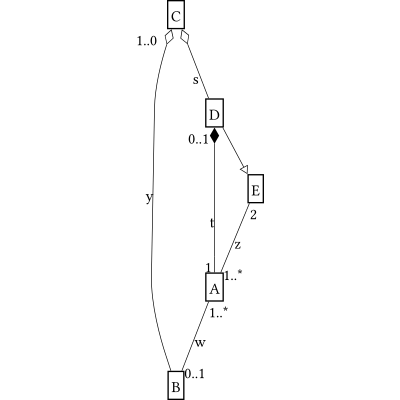
\includegraphics[min width=0.4\textwidth=0.6\textwidth,min height=0.4\textwidth=0.6\textwidth,keepaspectratio,max width=0.9\textwidth,max height=0.9\textwidth]{55/cd37ac6ad6ed2c227b4b30e91fae819c9c1cdefc064aad85ece210411452eaf1b801af83b04c596701db35357ce8aed00a3a92e08161.pdf}\end{centering}



Which of the following changes would each repair the class diagram?

\begin{enumerate}\item[ 1 ]{add a relationship that makes C a composition of Es where C participates exactly once and E participates exactly twice}
\item[ 2 ]{replace the inheritance where D inherits from E by an inheritance where E inherits from D}
\item[ 3 ]{replace aggregation y by a relationship that makes C a composition of Bs where C participates exactly once and B participates with the default multiplicity}
\item[ 4 ]{replace aggregation y by a relationship that makes C a composition of Bs where C participates 0..1 times and B participates with the default multiplicity}
\end{enumerate}Please state your answer by giving a list of numbers, indicating all changes each resulting in a valid class diagram.

Answer by giving a comma separated list of all appropriate options, e.g., \begin{verbatim}[1, 2]\end{verbatim} would indicate that options 1 and 2 each repair the given class diagram.

Please note: Classes are represented simplified here. 
 That means they consist of a single box containing only the class name but no sections for attributes or methods. 
 Nevertheless you should treat these simplified class representations as valid classes.

Please note: When hovering over or clicking on edges / nodes or their labels, the respective components that belong together are highlighted.

